\section{Clustering}
The clustering process begins with the generation of a dendrogram using Ward's method, which minimizes within-cluster variance and produces more balanced clusters. This approach is particularly suitable for customer segmentation as it identifies natural groupings based on similar characteristics.

\begin{figure}[H]
    \centering
    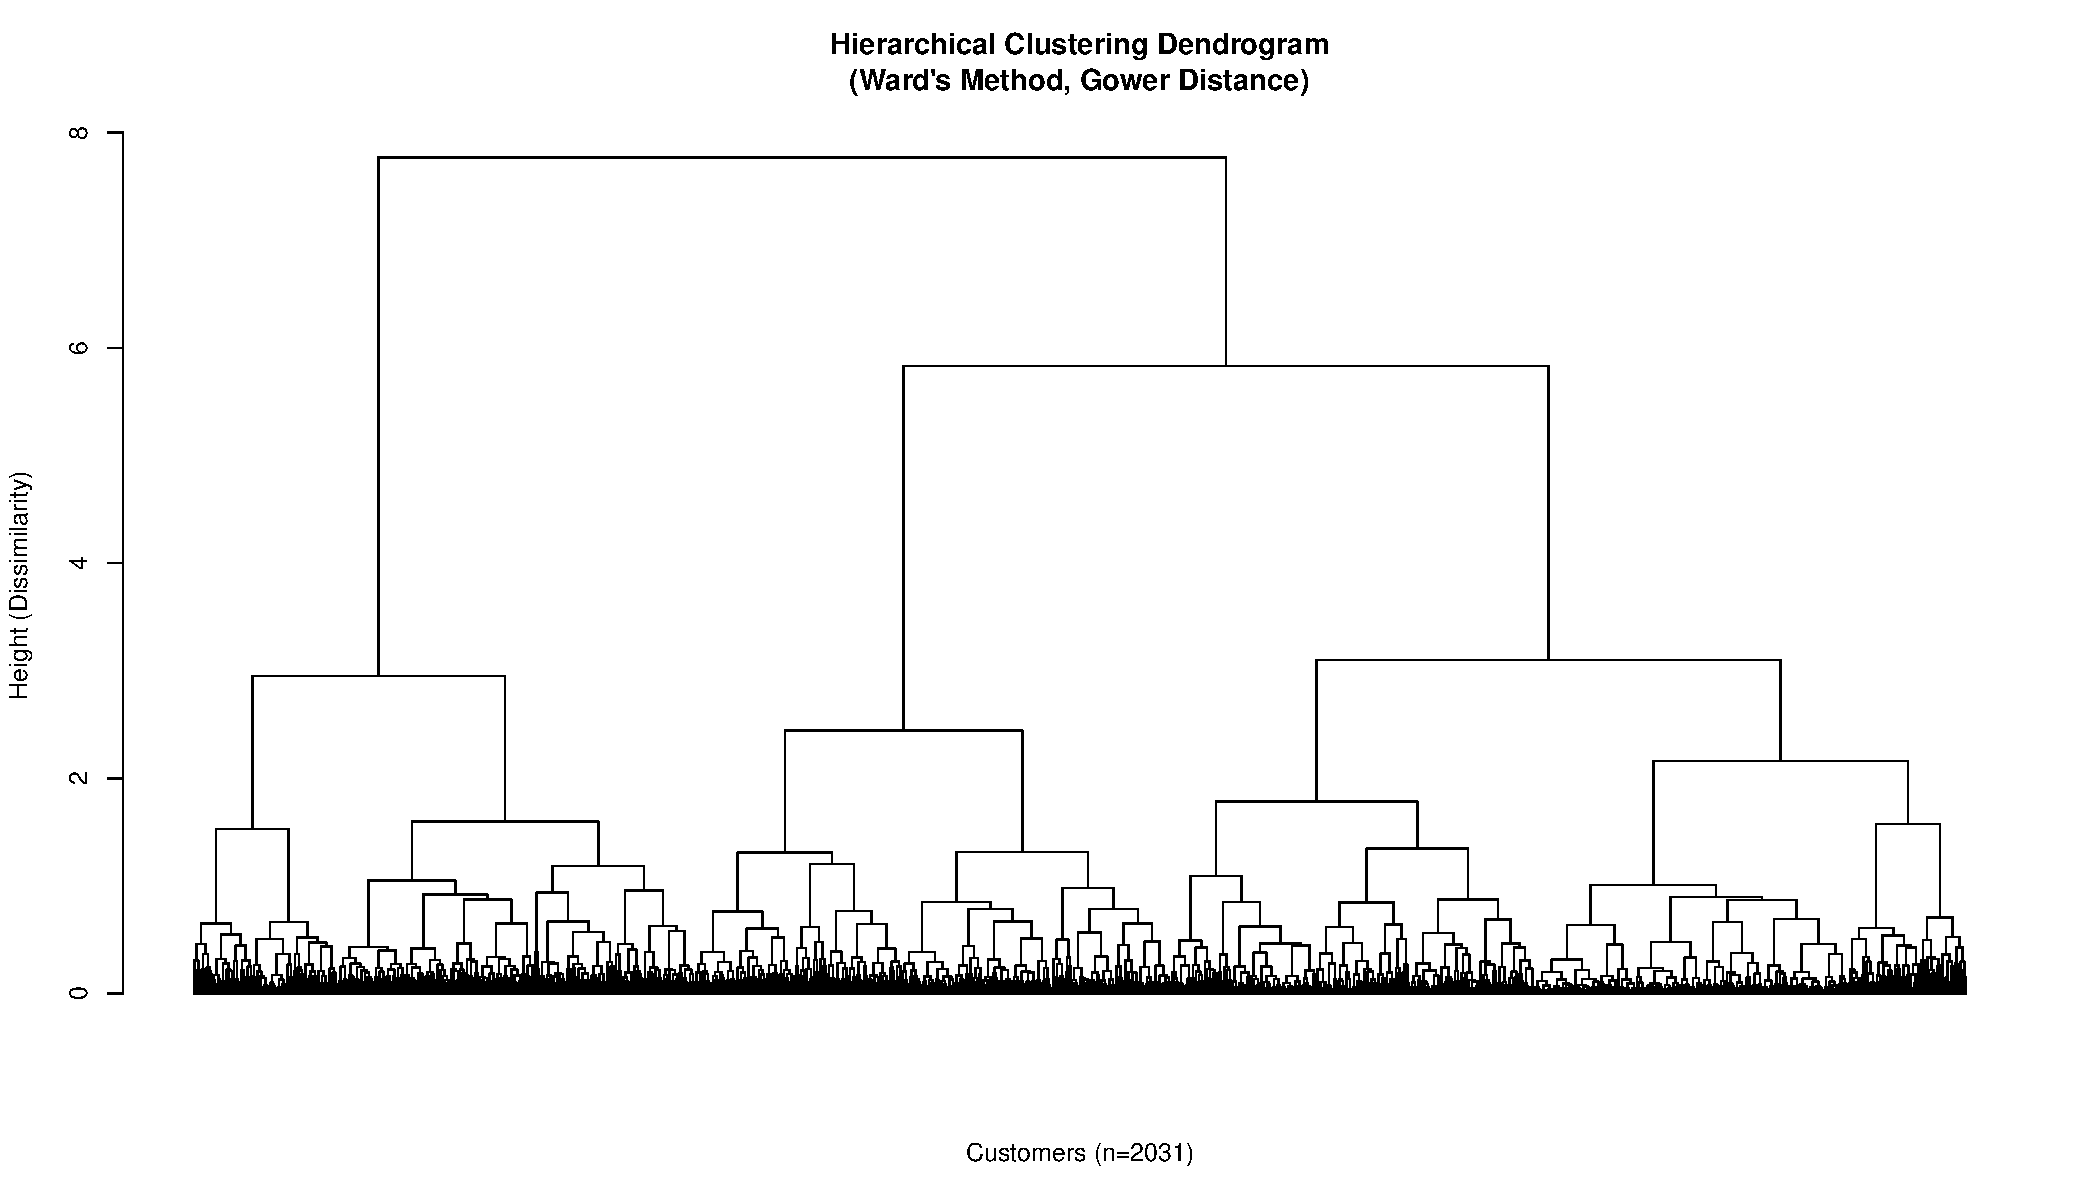
\includegraphics[width=1\linewidth]{Imatges/dendrogram_Gower_Ward.pdf}
    \caption{Dendrogram}
    \label{fig:dend}
\end{figure}

The analysis employed the Gower distance metric to accommodate both numerical variables (income, age, purchase frequency) and categorical variables (education level, marital status) in the dataset. This metric is particularly valuable for mixed data types as it standardizes different variable types into a unified dissimilarity matrix.

Using the elbow method and silhouette analysis shown in Figure \ref{fig:optdig}, it was determined that $k = 3$ is the appropriate number of clusters. The elbow method examines the decrease in within-cluster variation as more clusters are added, with the "elbow" indicating the point of diminishing returns. While silhouette analysis suggested a potential optimum at k = 2, the elbow method showed a notable bend at k = 3, providing better granularity for marketing objectives without over-fragmenting the customer base.

\begin{figure}[H]
    \centering
    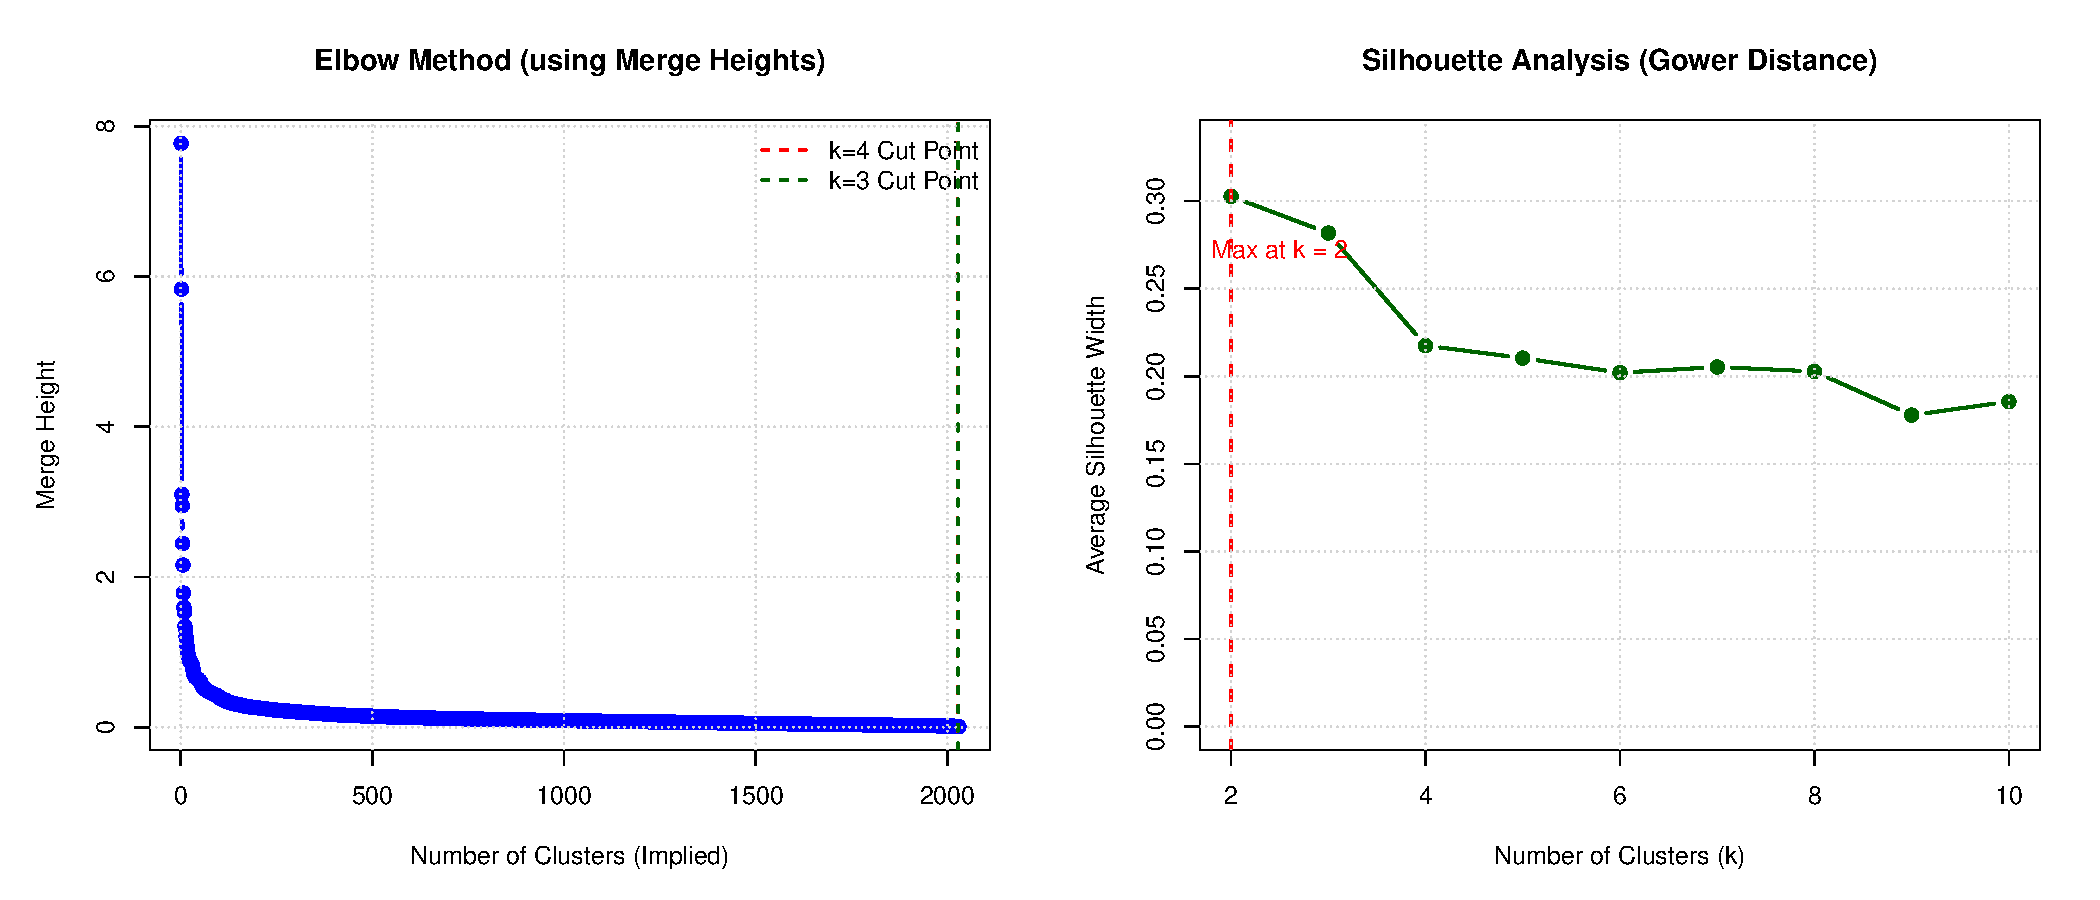
\includegraphics[width=1\linewidth]{Imatges/Clustering_OptimalK_Diagnostics_Gower.pdf}
    \caption{Clustering Optimal Diagnostics}
    \label{fig:optdig}
\end{figure}

The three clusters identified represent distinct customer segments, visualized in Figure \ref{fig:cdend}. Selecting three clusters strikes a balance between statistical validity and practical interpretability—ensuring segments are both mathematically distinct and actionable from a marketing perspective.

\begin{figure}[H]
    \centering
    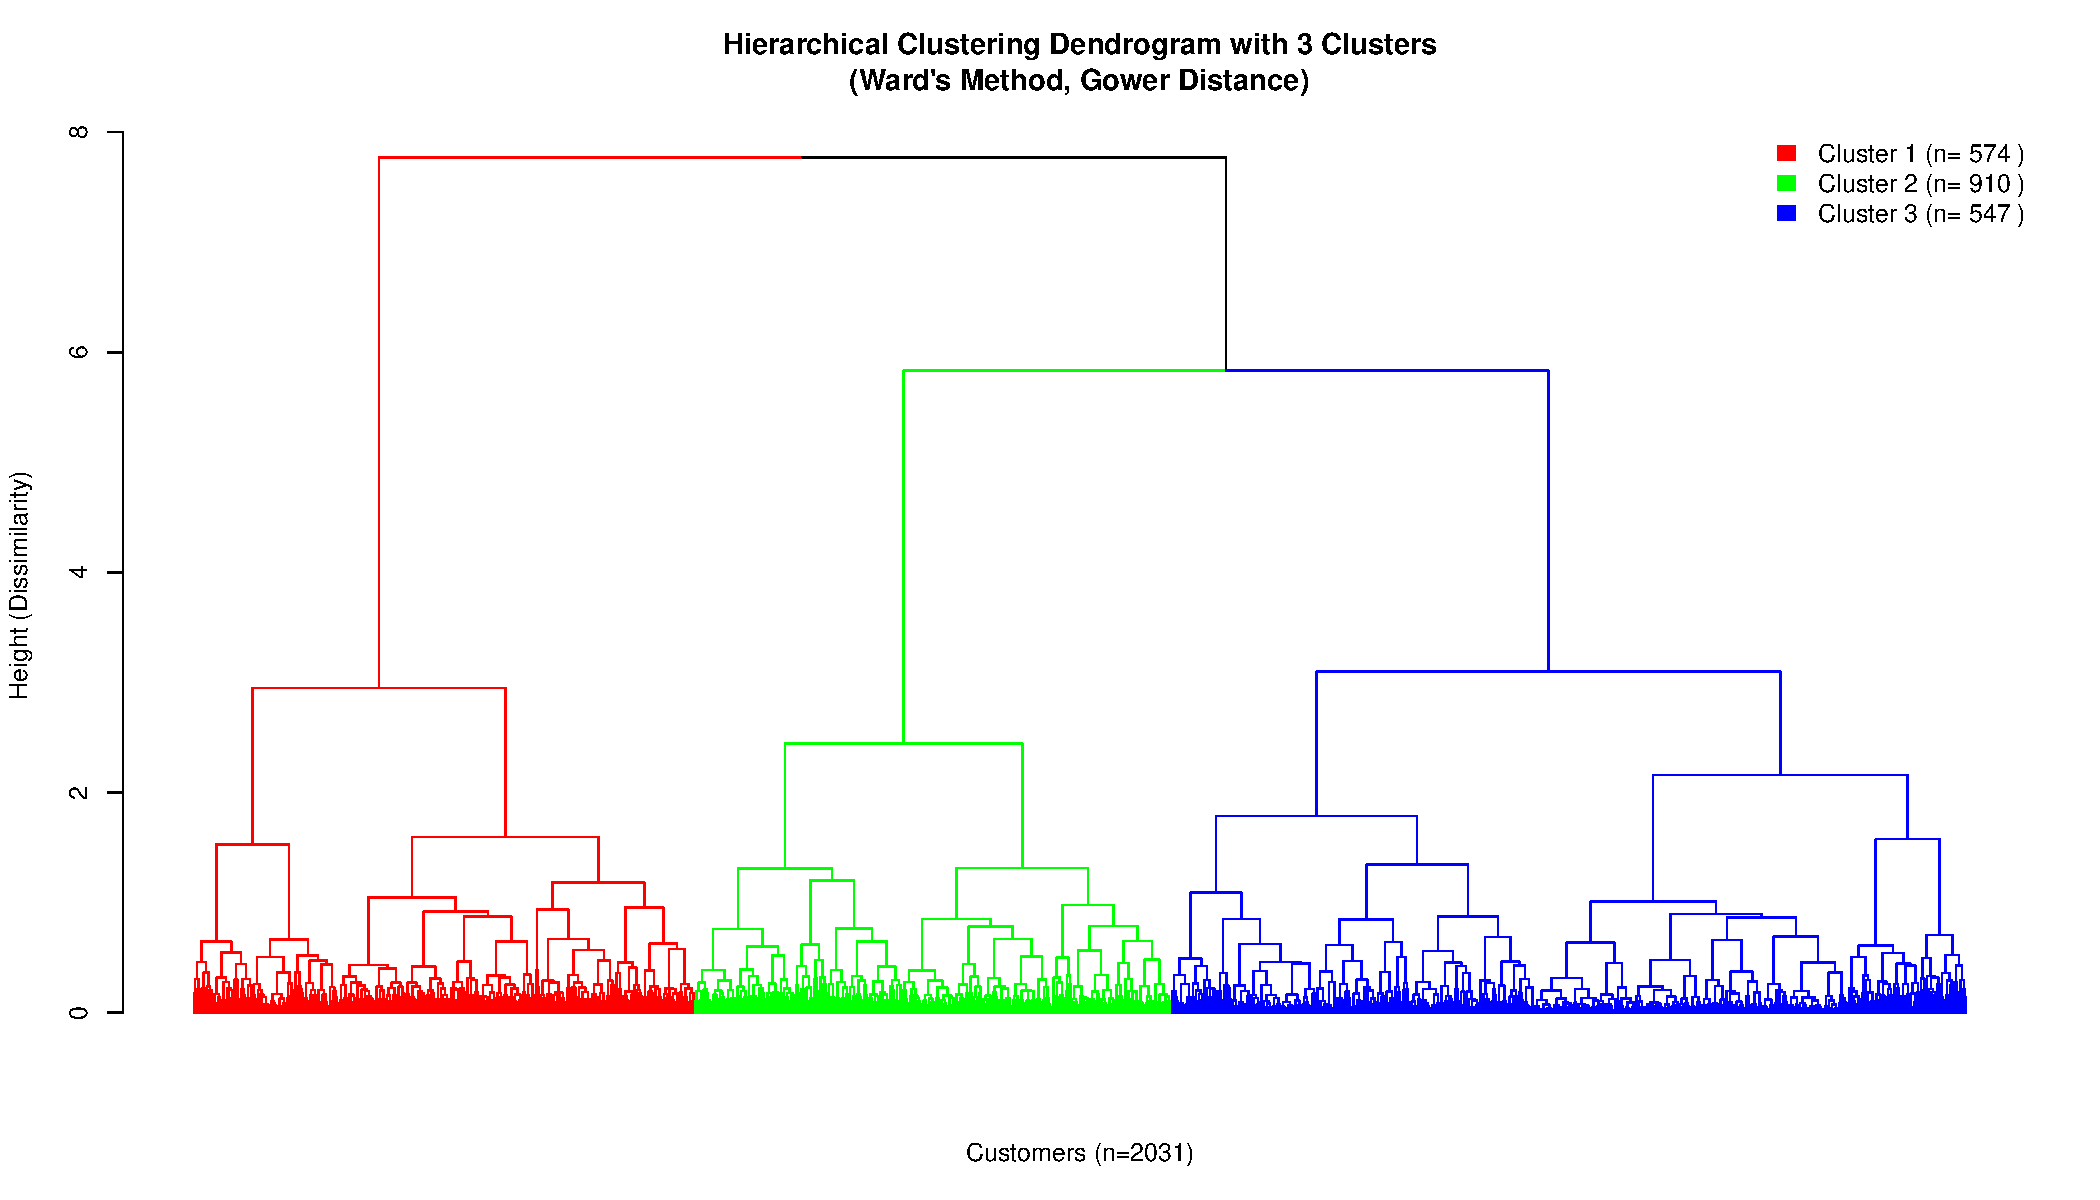
\includegraphics[width=1\linewidth]{Imatges/dendrogram_Gower_Ward_Colored.pdf}
    \caption{Coloured Dendrogram}
    \label{fig:cdend}
\end{figure}
